%%%%%%%%%%%%%%%%%%%%%%%%%%%%%%%%%%%%%%%%%
% Beamer Presentation - Báo cáo thực tập 2
% Theme + convention theo template presentation_1.tex (Madrid)
%%%%%%%%%%%%%%%%%%%%%%%%%%%%%%%%%%%%%%%%%

%----------------------------------------------------------------------------------------
%	PACKAGES AND THEMES
%----------------------------------------------------------------------------------------

\documentclass{beamer}

\mode<presentation> {
\usepackage{vntex}
\usetheme{Madrid}
}

\usepackage{graphicx} % Allows including images
\usepackage{booktabs} % Allows the use of \toprule, \midrule and \bottomrule in tables
\usepackage{multirow} % gộp ô theo nhóm trong bảng chi tiết
\usepackage{tikz} % Sơ đồ pipeline tổng quát
\usepackage[sorting=none,backend=biber]{biblatex}
\addbibresource{thesiscite.bib}

\usepackage[utf8]{inputenc}

\setbeamertemplate{footline}
{%
  \leavevmode%
  \hbox{%
  \begin{beamercolorbox}[wd=.333333\paperwidth,ht=2.25ex,dp=1ex,center]{author in head/foot}%
    \usebeamerfont{title in head/foot}\insertshorttitle
  \end{beamercolorbox}%
  \begin{beamercolorbox}[wd=.333333\paperwidth,ht=2.25ex,dp=1ex,center]{title in head/foot}%
    \usebeamerfont{title in head/foot}\insertsectionhead
  \end{beamercolorbox}%
  \begin{beamercolorbox}[wd=.333333\paperwidth,ht=2.25ex,dp=1ex,leftskip=2ex,rightskip=2ex,sep=0pt]{date in head/foot}%
    \hfill%
    \usebeamerfont{date in head/foot}%
    \insertshortdate{}%
    \hfill%
    \usebeamercolor[fg]{page number in head/foot}%
    \usebeamerfont{page number in head/foot}%
    \usebeamertemplate{page number in head/foot}%
  \end{beamercolorbox}}%
  \vskip0pt%
}
\setbeamertemplate{caption}[numbered]
\numberwithin{figure}{section}
\numberwithin{table}{section}

%----------------------------------------------------------------------------------------
%	TITLE PAGE
%----------------------------------------------------------------------------------------

\title[Gán nhãn y tế cột sống]{ỨNG DỤNG AI TRONG GÁN NHÃN Y TẾ CHO BỆNH ĐAU THẮT LƯNG}

\author{Hà Trung Kiên - 2470723}
\institute[HCMUT]
{
\textit{Giảng viên hướng dẫn} \\
TS. Phan Trọng Nhân \\
\medskip
\medskip
\medskip
Đại học Quốc gia Thành phố Hồ Chí Minh \\
Trường Đại học Bách Khoa \\
\medskip
\textit{Báo cáo thực tập tốt nghiệp}
}

\date{\today}
\begin{document}

\begin{frame}
\titlepage
\end{frame}

\begin{frame}
\frametitle{Mục lục}
\tableofcontents[hideallsubsections]
\end{frame}

%----------------------------------------------------------------------------------------
%	1. GIỚI THIỆU
%----------------------------------------------------------------------------------------
\section{Giới thiệu}
{
    \begin{frame}
        \frametitle{Mục lục}
        \tableofcontents[currentsection, hideothersubsections]
    \end{frame}
}

\subsection{Giới thiệu đề tài}
\begin{frame}
\frametitle{Giới thiệu đề tài}
\begin{itemize}
    \item[--] Đau thắt lưng là bệnh lý rất phổ biến; chẩn đoán dựa nhiều vào việc bác sĩ đọc thủ công ảnh MRI cột sống.
    \pause
    \item[--] Việc đọc thủ công tốn thời gian, phụ thuộc kinh nghiệm và dễ bỏ sót các ca nặng.
    \pause
    \item[$\rightarrow$] Cần một hệ thống AI hỗ trợ tự động: vừa phân vùng cấu trúc giải phẫu, vừa phát hiện và đánh giá các dấu hiệu bất thường.
\end{itemize}
\end{frame}

\begin{frame}
\frametitle{Ví dụ các dấu hiệu bất thường}
\begin{figure}
    \centering
    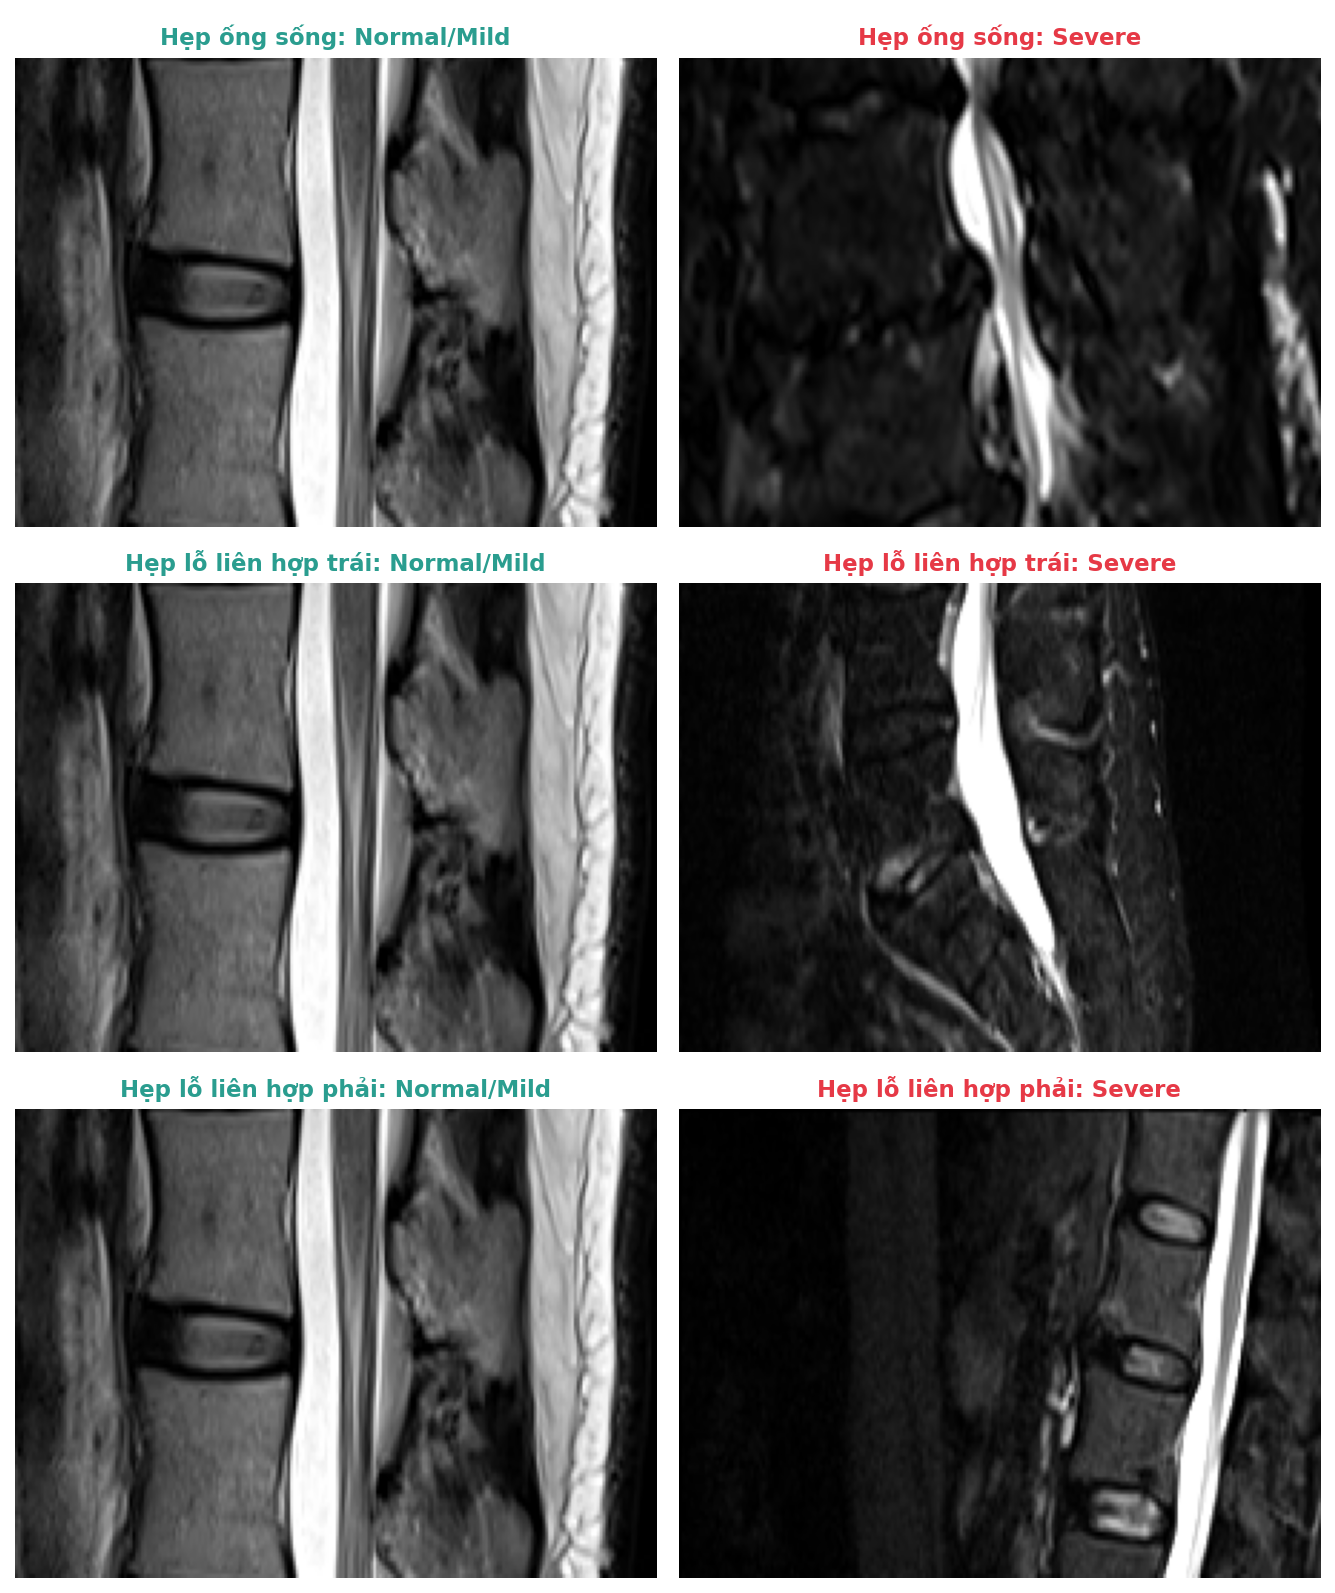
\includegraphics[height=0.76\textheight]{image/abnormality_examples.png}
    \caption{Normal/Mild so với Severe cho 3 nhóm bệnh lý (RSNA 2024).}
\end{figure}
\end{frame}

\subsection{Mục tiêu và phạm vi}
\begin{frame}
\frametitle{Mục tiêu đề tài}
\begin{itemize}
    \item[--] Xây dựng pipeline xử lý ảnh MRI cột sống thắt lưng gồm hai giai đoạn: phân vùng cấu trúc giải phẫu và đánh giá bất thường.
    \item[--] Khảo sát, lựa chọn mô hình tham khảo phù hợp cho từng giai đoạn.
    \item[--] Đề xuất kiến trúc tinh chỉnh mô-đun grading nhằm cải thiện điểm yếu trên lớp bệnh nặng (Severe).
    \item[--] Kiểm chứng khả năng tổng quát hóa qua transfer learning sang bộ dữ liệu khác.
\end{itemize}
\end{frame}

\begin{frame}
\frametitle{Phạm vi đề tài}
\begin{itemize}
    \item[--] \textbf{Dữ liệu:} chỉ ảnh MRI cột sống thắt lưng (không xử lý X-quang/CT), chủ yếu mặt cắt Sagittal T2/STIR; chưa khai thác mặt cắt Axial.
    \item[--] \textbf{Cấu trúc giải phẫu:} đốt sống, đĩa đệm, ống sống và tủy sống.
    \item[--] \textbf{Bệnh lý đánh giá:} hẹp ống sống, hẹp lỗ liên hợp trái/phải (RSNA); mở rộng sang Pfirrmann, Modic, thoát vị, phồng đĩa đệm, trượt đốt sống (SPIDER).
\end{itemize}
\pause
\textbf{Phạm vi giai đoạn thực tập:}
\begin{itemize}
    \item[--] Là bước tiền đề của Đồ án tốt nghiệp, tập trung lựa chọn mô hình và tinh chỉnh mô-đun grading.
    \item[$\rightarrow$] Tích hợp pipeline hoàn chỉnh và phần mềm giao diện được đưa vào kế hoạch Đồ án tốt nghiệp.
\end{itemize}
\end{frame}

%----------------------------------------------------------------------------------------
%	2. CÔNG TRÌNH LIÊN QUAN
%----------------------------------------------------------------------------------------
\section{Công trình nghiên cứu liên quan}
{
    \begin{frame}
        \frametitle{Mục lục}
        \tableofcontents[currentsection, hideothersubsections]
    \end{frame}
}

\subsection{Phân vùng cấu trúc giải phẫu}
\begin{frame}
\frametitle{Các phương pháp phân vùng cột sống}
\begin{itemize}
    \item[--] \textbf{SpineSegDiff}~\cite{monzon2024diffusion}: mô hình khuếch tán. Thay vì khử nhiễu từ nhiễu Gaussian, dùng mặt nạ thô của nnU-Net~\cite{isensee2021nnunet} làm điểm khởi đầu rồi tinh chỉnh qua vài bước khuếch tán, cho biên đĩa đệm mịn hơn.
    \pause
    \item[--] \textbf{TotalSpineSeg}~\cite{warszawer2025totalspineseg}: hai nnU-Net nối tiếp -- mô hình thứ nhất định vị các đĩa đệm cột mốc, mô hình thứ hai phân vùng và gán nhãn chi tiết toàn cột sống (đốt sống, đĩa đệm, tủy sống).
    \pause
    \item[--] \textbf{SPINEPS}~\cite{moller2024spineps}: hai pha -- pha ngữ nghĩa phân vùng các lớp mô, pha thực thể tách riêng từng đốt sống thành các cá thể độc lập.
    \pause
    \item[--] \textbf{MedCLIP-SAMv2}~\cite{koleilat2025medclipsamv2}: zero-shot -- dùng BiomedCLIP định vị vùng theo câu lệnh văn bản, sau đó SAM sinh mặt nạ chi tiết mà không cần dữ liệu gán nhãn.
\end{itemize}
\end{frame}

\subsection{Đánh giá bất thường}
\begin{frame}
\frametitle{Các phương pháp đánh giá bất thường}
\begin{itemize}
    \item[--] \textbf{SpineNetV2}~\cite{windsor2022spinenetv2}: phát hiện đốt sống bằng VFR, trích xuất khối ảnh 3D quanh đĩa đệm rồi đưa qua CNN 3D đa nhánh.
    \begin{itemize}\item[$\circ$] Đánh giá 8--10 nhãn cùng lúc, mã nguồn mở; phụ thuộc bước phát hiện và mới dùng mặt cắt Sagittal.\end{itemize}
    \pause
    \item[--] \textbf{MedGemma}~\cite{google2025medgemma}: mô hình Ngôn ngữ--Thị giác lớn, đánh giá theo dạng hỏi--đáp zero-shot.
    \begin{itemize}\item[$\circ$] Rất linh hoạt nhưng chỉ phân loại, không định vị; Recall thấp trên cột sống thắt lưng.\end{itemize}
    \pause
    \item[--] \textbf{Ning Shen (RSNA 2024)}~\cite{nshen7_rsna2024}: kiến trúc segmentation rồi classification, giải pháp top Kaggle.
    \begin{itemize}\item[$\circ$] Hiệu năng cao nhưng chỉ 5 nhãn và mới công bố trên Kaggle, chưa được thẩm định qua bình duyệt khoa học (peer-review).\end{itemize}
\end{itemize}
\end{frame}

%----------------------------------------------------------------------------------------
%	3. DỮ LIỆU VÀ LỰA CHỌN MÔ HÌNH
%----------------------------------------------------------------------------------------
\section{Dữ liệu và lựa chọn mô hình}
{
    \begin{frame}
        \frametitle{Mục lục}
        \tableofcontents[currentsection, hideothersubsections]
    \end{frame}
}

\subsection{Bộ dữ liệu}
\begin{frame}
\frametitle{Bộ dữ liệu}
\begin{itemize}
    \item[--] \textbf{RSNA 2024}~\cite{rsna2024dataset}: 3 nhãn (hẹp ống sống, hẹp lỗ liên hợp trái/phải).
    \pause
    \item[--] \textbf{SPIDER}~\cite{vansluijs2022spider}: 8 nhãn (Pfirrmann, Modic, herniation, bulging, \ldots) dùng kiểm chứng tổng quát hóa.
    \pause
    \item[$\rightarrow$] Cả hai bộ đều mất cân bằng lớp nghiêm trọng, lớp bệnh nặng chiếm tỉ lệ rất nhỏ.
\end{itemize}
\end{frame}

\begin{frame}
\frametitle{Phân bố lớp trên RSNA 2024}
\begin{figure}
    \centering
    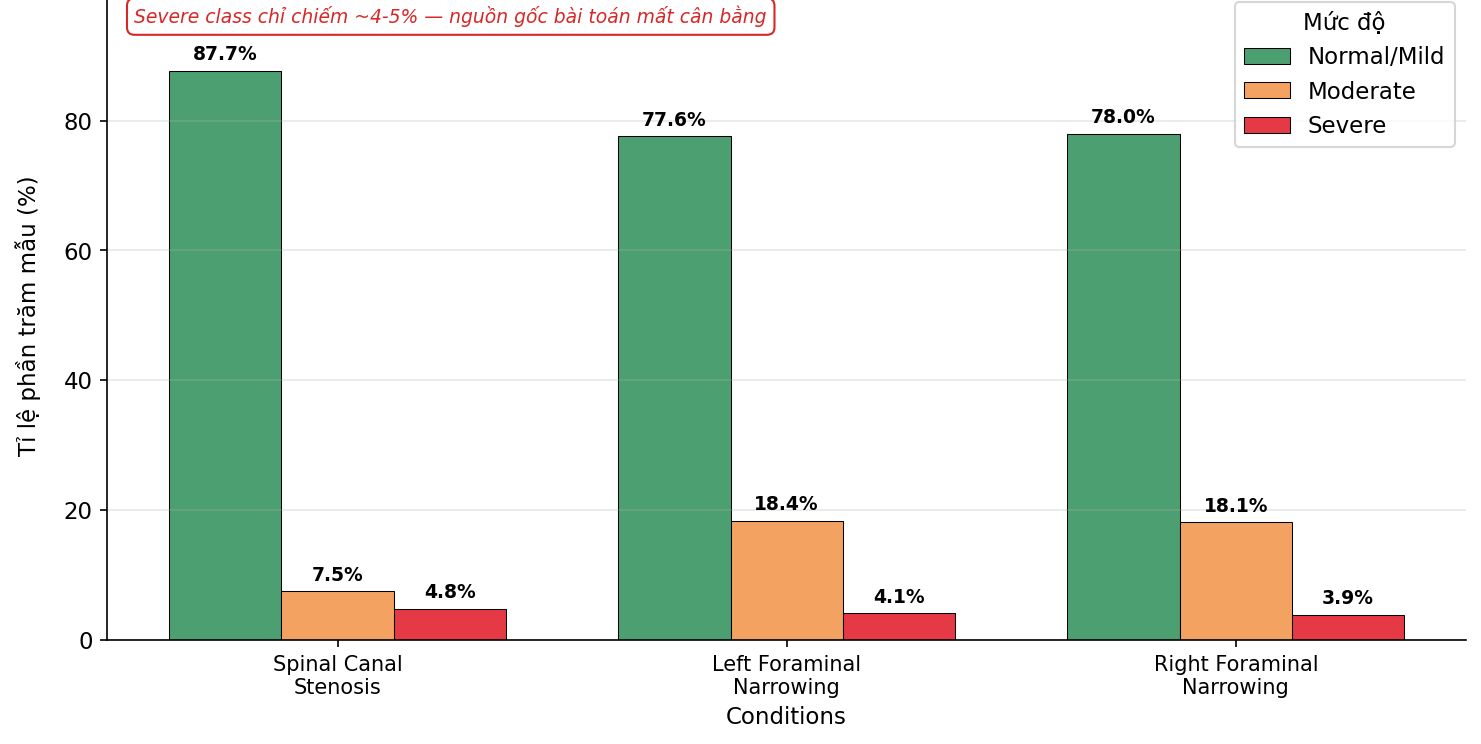
\includegraphics[width=0.9\textwidth]{image/rsna_class_distribution.png}
    \caption{Phân bố lớp trên RSNA 2024.}
\end{figure}
\end{frame}

\begin{frame}
\frametitle{Phân bố nhãn trên SPIDER}
\begin{figure}
    \centering
    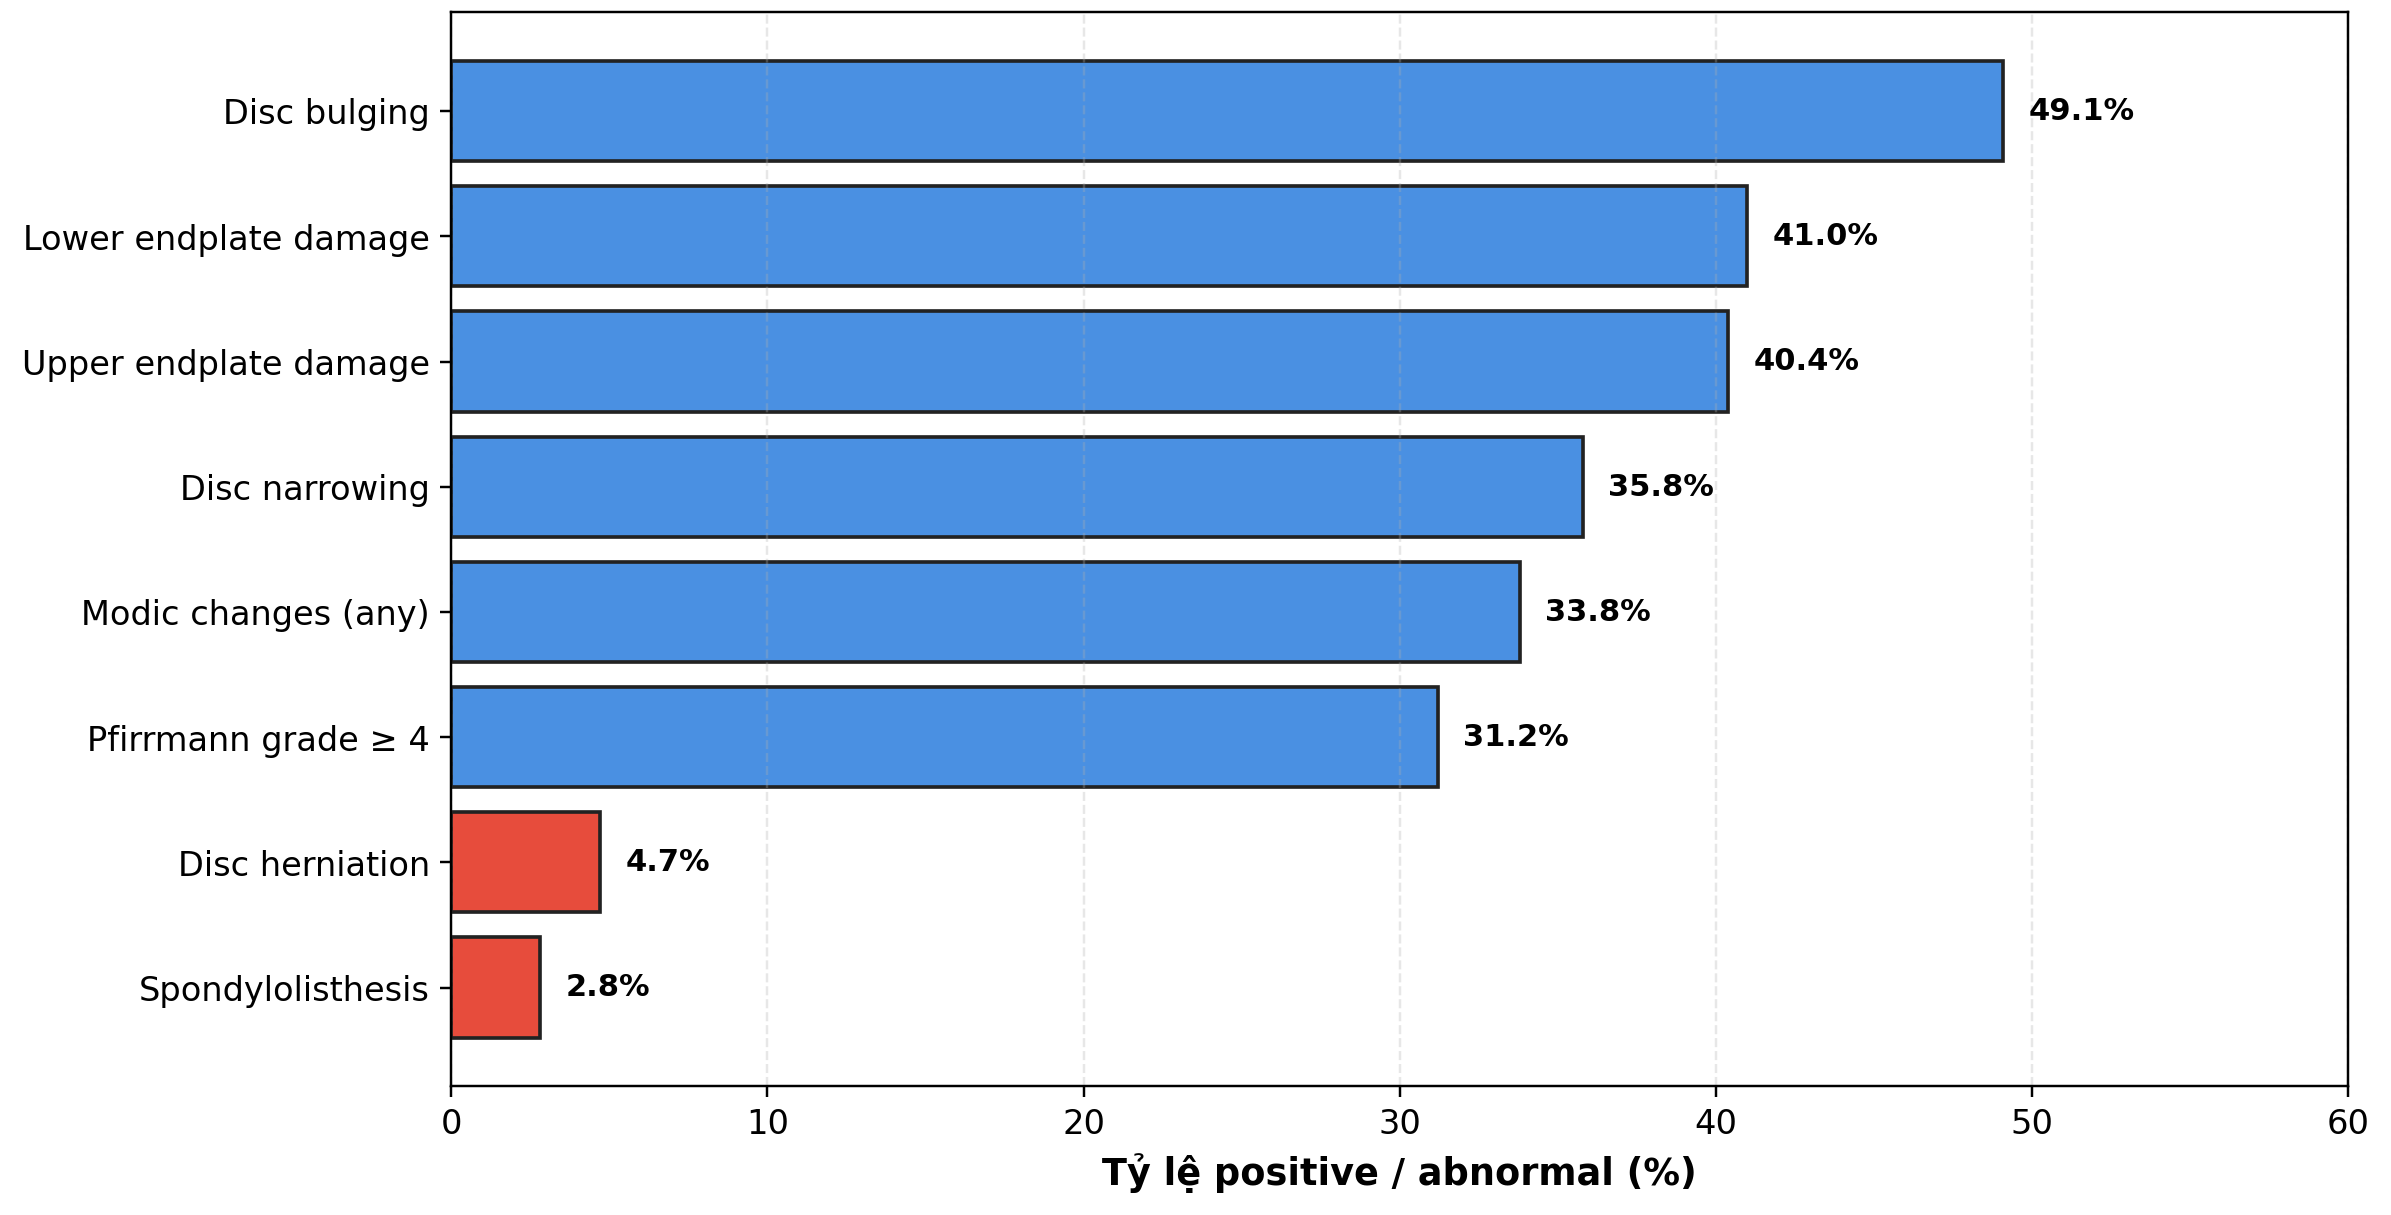
\includegraphics[width=0.82\textwidth]{image/spider_class_distribution.png}
    \caption{Phân bố nhãn trên SPIDER 8 conditions.}
\end{figure}
\end{frame}

\subsection{Lựa chọn mô hình tham khảo}
\begin{frame}
\frametitle{Lựa chọn mô hình phân vùng}
\begin{table}
\centering
\small
\begin{tabular}{lcccc}
\toprule
\textbf{Tiêu chí} & \textbf{TotalSpineSeg} & \textbf{SPINEPS} & \textbf{MedCLIP-SAMv2} & \textbf{SpineNetV2} \\
\midrule
Dice Score & \textbf{70.81\%} & 58.68\% & 40.55\% & 67.82\% \\
Precision  & \textbf{97.87\%} & 52.17\% & 29.16\% & 51.76\% \\
Recall     & 56.49\% & 68.34\% & \textbf{91.98\%} & 91.79\% \\
ASSD       & \textbf{6.85 mm} & 7.48 mm & 19.50 mm & 8.04 mm \\
\bottomrule
\end{tabular}
\caption{So sánh hiệu năng phân vùng giữa bốn mô hình tham khảo.}
\end{table}
\begin{itemize}
    \item[$\rightarrow$] Chọn TotalSpineSeg: Precision 97.87\% và ASSD thấp nhất, định vị thân đốt sống chính xác để trích xuất ROI.
\end{itemize}
\end{frame}

\begin{frame}
\frametitle{Lựa chọn mô hình đánh giá}
\begin{table}
\centering
\begin{tabular}{lccc}
\toprule
\textbf{Nhóm bệnh (F1)} & \textbf{Ning Shen} & \textbf{SpineNetV2} & \textbf{MedGemma} \\
\midrule
Hẹp ống sống          & 81.20\% & 78.79\% & 31.17\% \\
Hẹp lỗ liên hợp trái  & 79.43\% & 77.30\% & 13.86\% \\
Hẹp lỗ liên hợp phải  & 81.48\% & 76.40\% & 10.75\% \\
\bottomrule
\end{tabular}
\caption{So sánh F1 phát hiện bất thường trên ba nhóm bệnh.}
\end{table}
\begin{itemize}
    \item[$\rightarrow$] Chọn SpineNetV2 làm backbone (chuyên biệt cột sống, nhiều nhãn); MedGemma có Recall rất thấp (6--21\%) do chưa chuyên biệt hóa.
\end{itemize}
\end{frame}

%----------------------------------------------------------------------------------------
%	4. MÔ HÌNH ĐỀ XUẤT
%----------------------------------------------------------------------------------------
\section{Mô hình đề xuất}
{
    \begin{frame}
        \frametitle{Mục lục}
        \tableofcontents[currentsection, hideothersubsections]
    \end{frame}
}

\subsection{Kiến trúc tổng thể}
\begin{frame}
\frametitle{Pipeline tổng thể của giải pháp}
\begin{figure}
\centering
\resizebox{\textwidth}{!}{%
\begin{tikzpicture}[
    box/.style={rectangle, draw=blue!70, fill=blue!8, rounded corners, minimum width=1.9cm, minimum height=0.95cm, align=center, font=\footnotesize, thick},
    dataout/.style={rectangle, draw=green!50!black, fill=green!12, rounded corners, minimum width=1.9cm, minimum height=0.95cm, align=center, font=\footnotesize, thick},
    plan/.style={rectangle, draw=gray, dashed, fill=gray!8, rounded corners, minimum width=2.0cm, minimum height=0.95cm, align=center, font=\footnotesize, thick},
    a/.style={->, thick, blue!70!black},
    pa/.style={->, thick, gray, dashed}
]
    \node[box] (in)   at (0,0)    {Ảnh MRI};
    \node[box] (seg)  at (2.6,0)  {Phân vùng\\\scriptsize TotalSpineSeg};
    \node[dataout] (mask) at (5.2,0)  {Mặt nạ};
    \node[box] (gr)   at (7.8,0)  {Đánh giá\\\scriptsize Hybrid grading};
    \node[dataout] (lb)   at (10.4,0) {Nhãn bệnh lý};
    \node[plan](sw)   at (13.0,0) {Phần mềm\\\scriptsize giao diện};
    \draw[a] (in) -- (seg);
    \draw[a] (seg) -- (mask);
    \draw[pa] (mask) -- node[above,font=\scriptsize,text=gray]{ROI} (gr);
    \draw[a] (gr) -- (lb);
    \draw[pa] (lb) -- (sw);
    \draw[a] (in) to[bend right=30] node[below,font=\scriptsize]{TT2: ảnh MRI trực tiếp} (gr);
\end{tikzpicture}}
\caption{Kiến trúc tổng thể: nét liền đã làm ở thực tập, nét đứt là kế hoạch Đồ án tốt nghiệp.}
\end{figure}
\begin{itemize}
    \item[--] Luồng mục tiêu tuần tự: MRI $\rightarrow$ phân vùng $\rightarrow$ mặt nạ định vị ROI $\rightarrow$ đánh giá $\rightarrow$ phần mềm.
    \item[--] Hiện trạng thực tập: hai mô-đun chạy độc lập, grading nhận ảnh MRI trực tiếp.
\end{itemize}
\end{frame}

\subsection{Động lực thiết kế}
\begin{frame}
\frametitle{Động lực: vì sao chọn CBAM + BiomedCLIP?}
\textbf{Vấn đề:} SpineNetV2 baseline bỏ sót gần 90\% ca Severe (Recall 11.5\%) do mất cân bằng lớp và vùng tổn thương rất nhỏ trong khối ảnh.
\begin{itemize}
    \item[--] \textbf{CBAM (cơ chế chú ý nhẹ):} vùng bệnh lý chiếm tỉ lệ rất nhỏ $\rightarrow$ CBAM giúp mô hình tự ``tập trung'' vào đúng kênh đặc trưng và vị trí không gian quan trọng, thay vì xử lý đều toàn ảnh.
    \item[--] \textbf{BiomedCLIP (mô hình nền y khoa):} pretrained trên 15M cặp ảnh--văn bản y khoa $\rightarrow$ cung cấp đặc trưng nền tổng quát, bù cho việc dữ liệu lớp Severe quá ít.
    \item[$\rightarrow$] \textbf{Kết hợp:} CBAM khai thác chi tiết 3D cục bộ, BiomedCLIP cung cấp ngữ nghĩa tổng quát; nhờ vậy vừa cải thiện Severe vừa tổng quát hóa tốt hơn từng mô hình đơn lẻ (kiểm chứng qua ablation).
\end{itemize}
\end{frame}

\subsection{Kiến trúc Hybrid hai nhánh}
\begin{frame}
\frametitle{Đóng góp chính: kiến trúc Hybrid hai nhánh}
\begin{columns}[c]
\column{.5\textwidth}
\begin{itemize}
    \item[--] \textbf{Nhánh CBAM-3D ResNet-34 (trainable):} học đặc trưng trực tiếp từ khối ảnh 3D đĩa đệm.
    \item[--] \textbf{Nhánh BiomedCLIP (frozen):} cung cấp prior tổng quát từ pretraining 15M cặp ảnh--văn bản y khoa.
    \item[--] Hai nhánh hợp nhất qua Fusion MLP, dẫn vào các head phân loại đa nhiệm.
\end{itemize}
\column{.5\textwidth}
\begin{figure}
    \centering
    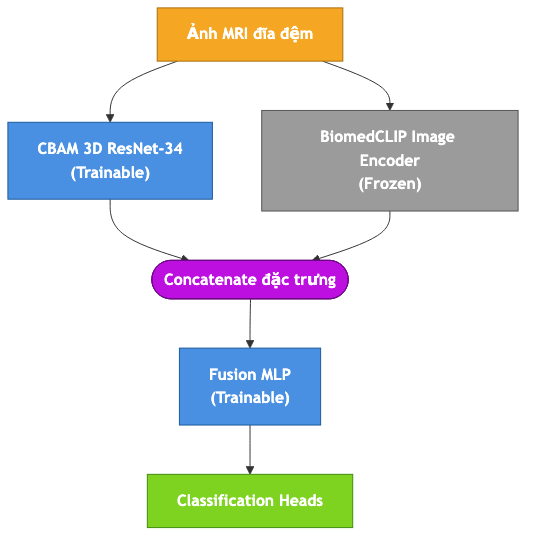
\includegraphics[width=\textwidth]{image/hybrid_architecture.png}
    \caption{Kiến trúc Hybrid hai nhánh.}
\end{figure}
\end{columns}
\end{frame}

\begin{frame}
\frametitle{Giai đoạn huấn luyện}
\begin{columns}[c]
\column{.5\textwidth}
\begin{itemize}
    \item[--] Dữ liệu qua augmentation và minority oversampling.
    \item[--] Gradient chỉ đi qua nhánh trainable (CBAM-ResNet); BiomedCLIP frozen hoàn toàn.
    \item[--] Chỉ 21.3M tham số được huấn luyện so với 86.2M tham số BiomedCLIP giữ cố định.
\end{itemize}
\column{.5\textwidth}
\begin{figure}
    \centering
    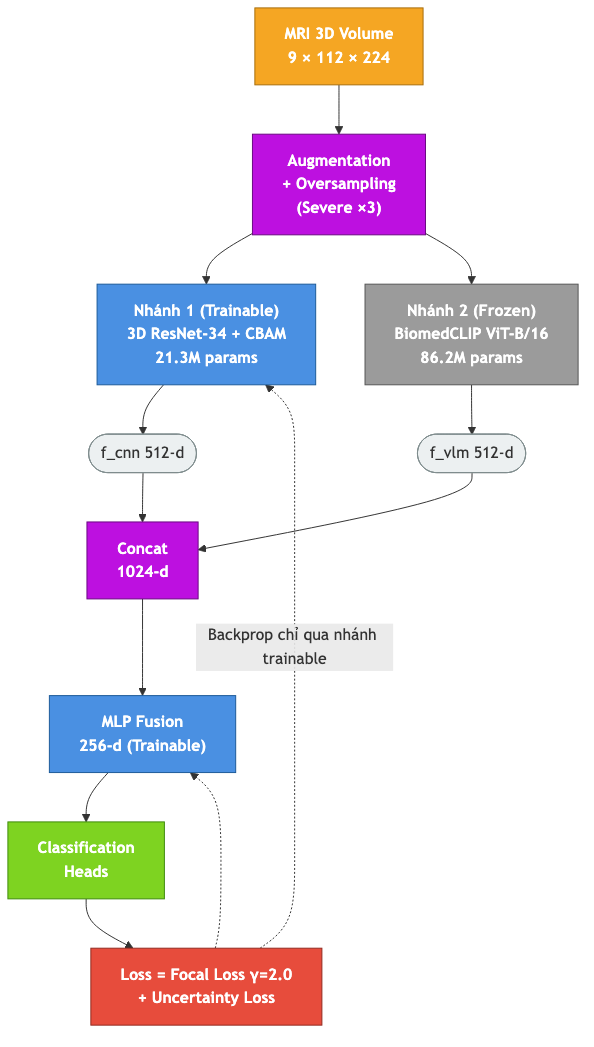
\includegraphics[height=0.82\textheight]{image/training_architecture.png}
    \caption{Kiến trúc giai đoạn huấn luyện.}
\end{figure}
\end{columns}
\end{frame}

\begin{frame}
\frametitle{Giai đoạn suy diễn}
\begin{columns}[c]
\column{.5\textwidth}
\begin{itemize}
    \item[--] Không augmentation, không tính loss; chỉ chạy forward pass.
    \item[--] Hai nhánh trích đặc trưng, hợp nhất rồi đưa qua các head sinh xác suất và nhãn dự đoán.
    \item[--] Thời gian suy diễn $\sim$66 ms/mẫu (NVIDIA RTX 4090).
\end{itemize}
\column{.5\textwidth}
\begin{figure}
    \centering
    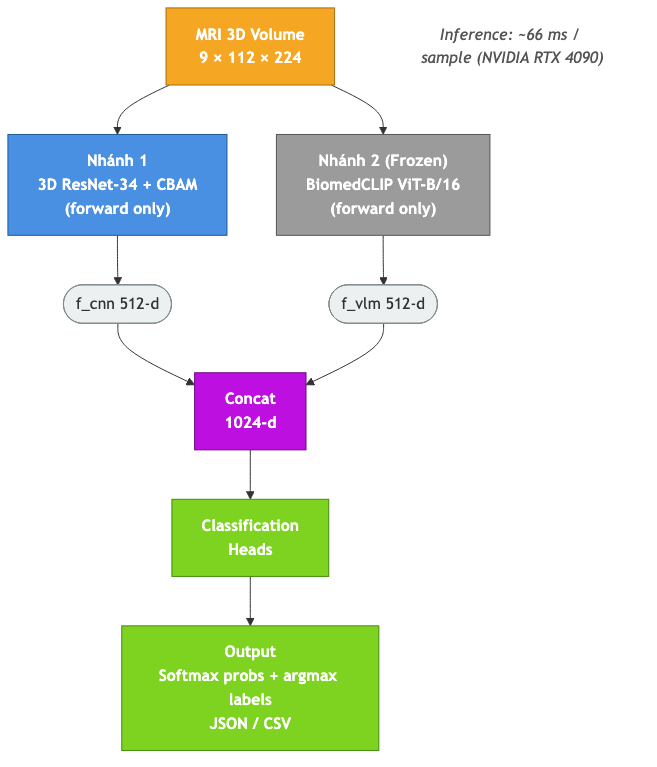
\includegraphics[height=0.82\textheight]{image/inference_architecture.png}
    \caption{Kiến trúc giai đoạn suy diễn.}
\end{figure}
\end{columns}
\end{frame}

\subsection{Xử lý mất cân bằng lớp}
\begin{frame}
\frametitle{Pipeline xử lý mất cân bằng lớp}
Phân bố nhãn rất lệch: Normal/Mild $\sim$78\%, Moderate $\sim$18\%, Severe chỉ $\sim$4\%.
\begin{itemize}
    \item[--] \textbf{Focal Loss}~\cite{lin2017focal}: giảm trọng số mẫu dễ, tăng cho mẫu khó (Severe).
    \item[--] \textbf{Uncertainty Loss}~\cite{kendall2018multitask}: học trọng số động giữa các nhiệm vụ.
    \item[--] \textbf{Minority oversampling:} lặp lại các mẫu chứa nhãn Severe.
\end{itemize}
\end{frame}

%----------------------------------------------------------------------------------------
%	5. KẾT QUẢ THỰC NGHIỆM
%----------------------------------------------------------------------------------------
\section{Kết quả thực nghiệm}
{
    \begin{frame}
        \frametitle{Mục lục}
        \tableofcontents[currentsection, hideothersubsections]
    \end{frame}
}

\subsection{Kết quả tinh chỉnh trên RSNA}
\begin{frame}
\frametitle{Kết quả tổng hợp trên RSNA 2024}
\begin{table}
\centering
\small
\begin{tabular}{lcccc}
\toprule
\textbf{Chỉ số} & \textbf{SpineNetV2} & \textbf{CBAM} & \textbf{BMC-only} & \textbf{Hybrid} \\
\midrule
Mean Accuracy   & \textbf{0.814} & 0.690 & 0.692 & 0.721 \\
Mean F1 (macro) & 0.420 & 0.502 & 0.464 & \textbf{0.528} \\
Mean AUC        & 0.826 & 0.822 & 0.812 & \textbf{0.837} \\
Mean AUPRC      & 0.523 & 0.519 & 0.482 & \textbf{0.526} \\
\midrule
\multicolumn{5}{l}{\textit{Lớp Severe (lớp focus lâm sàng)}} \\
Severe Recall   & 0.115 & 0.370 & 0.245 & \textbf{0.464} \\
Severe F1       & 0.149 & 0.304 & 0.229 & \textbf{0.343} \\
Severe AUC      & 0.860 & 0.886 & 0.874 & \textbf{0.896} \\
Severe AUPRC    & 0.276 & 0.319 & 0.218 & \textbf{0.321} \\
\bottomrule
\end{tabular}
\caption{Kết quả trung bình và lớp Severe của 4 cấu hình trên RSNA 2024.}
\end{table}
\begin{itemize}
    \item[$\rightarrow$] SpineNetV2 cao nhất ở Accuracy (do thiên về lớp đa số); Hybrid đánh đổi $\sim$9\% Accuracy để dẫn đầu F1/AUC/AUPRC và đặc biệt là lớp Severe (xem chi tiết bên dưới).
\end{itemize}
\end{frame}

\begin{frame}
\frametitle{Kết quả chi tiết theo lớp trên RSNA 2024}
\begin{table}
\centering
\scriptsize
\setlength{\tabcolsep}{4pt}
\renewcommand{\arraystretch}{1.05}
\begin{tabular}{llccccc}
\toprule
\textbf{Lớp} & \textbf{Cấu hình} & R & P & F1 & AUC & AUPRC \\
\midrule
\multirow{4}{*}{Normal/Mild}
 & SpineNetV2 & \textbf{0.963} & 0.840 & \textbf{0.897} & 0.829 & 0.948 \\
 & CBAM       & 0.693 & \textbf{0.949} & 0.791 & 0.848 & 0.949 \\
 & BMC-only   & 0.709 & 0.934 & 0.801 & 0.828 & 0.950 \\
 & Hybrid     & 0.746 & 0.937 & 0.825 & \textbf{0.861} & \textbf{0.957} \\
\midrule
\multirow{4}{*}{Moderate}
 & SpineNetV2 & 0.173 & \textbf{0.424} & 0.240 & \textbf{0.790} & \textbf{0.345} \\
 & CBAM       & \textbf{0.652} & 0.310 & 0.411 & 0.732 & 0.288 \\
 & BMC-only   & 0.563 & 0.280 & 0.360 & 0.733 & 0.278 \\
 & Hybrid     & 0.564 & 0.341 & \textbf{0.415} & 0.753 & 0.300 \\
\midrule
\multirow{4}{*}{\textbf{Severe}}
 & SpineNetV2 & 0.115 & 0.212 & 0.149 & 0.860 & 0.276 \\
 & CBAM       & 0.370 & 0.272 & 0.304 & 0.886 & 0.319 \\
 & BMC-only   & 0.245 & 0.211 & 0.229 & 0.874 & 0.218 \\
 & Hybrid     & \textbf{0.464} & \textbf{0.273} & \textbf{0.343} & \textbf{0.896} & \textbf{0.321} \\
\bottomrule
\end{tabular}
\caption{Chi tiết per-class trên RSNA 2024.}
\end{table}
\begin{itemize}
    \item[$\rightarrow$] Lớp Severe: Hybrid thắng cả 5 chỉ số, Severe Recall 11.5\% $\to$ 46.4\% (gấp $\sim$4 lần).
\end{itemize}
\end{frame}

\subsection{Khả năng diễn giải}
\begin{frame}
\frametitle{Trực quan hóa vùng chú ý (Grad-CAM)}
\begin{itemize}
    \item[--] Grad-CAM tô màu vùng ảnh ảnh hưởng nhiều nhất đến quyết định của mô hình (vùng càng nóng, mô hình càng chú ý).
    \item[--] Trên các ca Severe, vùng nóng trùng với vị trí tổn thương thật $\rightarrow$ mô hình ``nhìn'' đúng chỗ, tăng độ tin cậy và khả năng diễn giải cho bác sĩ.
\end{itemize}
\end{frame}

\begin{frame}
\frametitle{Trực quan hóa vùng chú ý (Grad-CAM)}
\begin{figure}
    \centering
    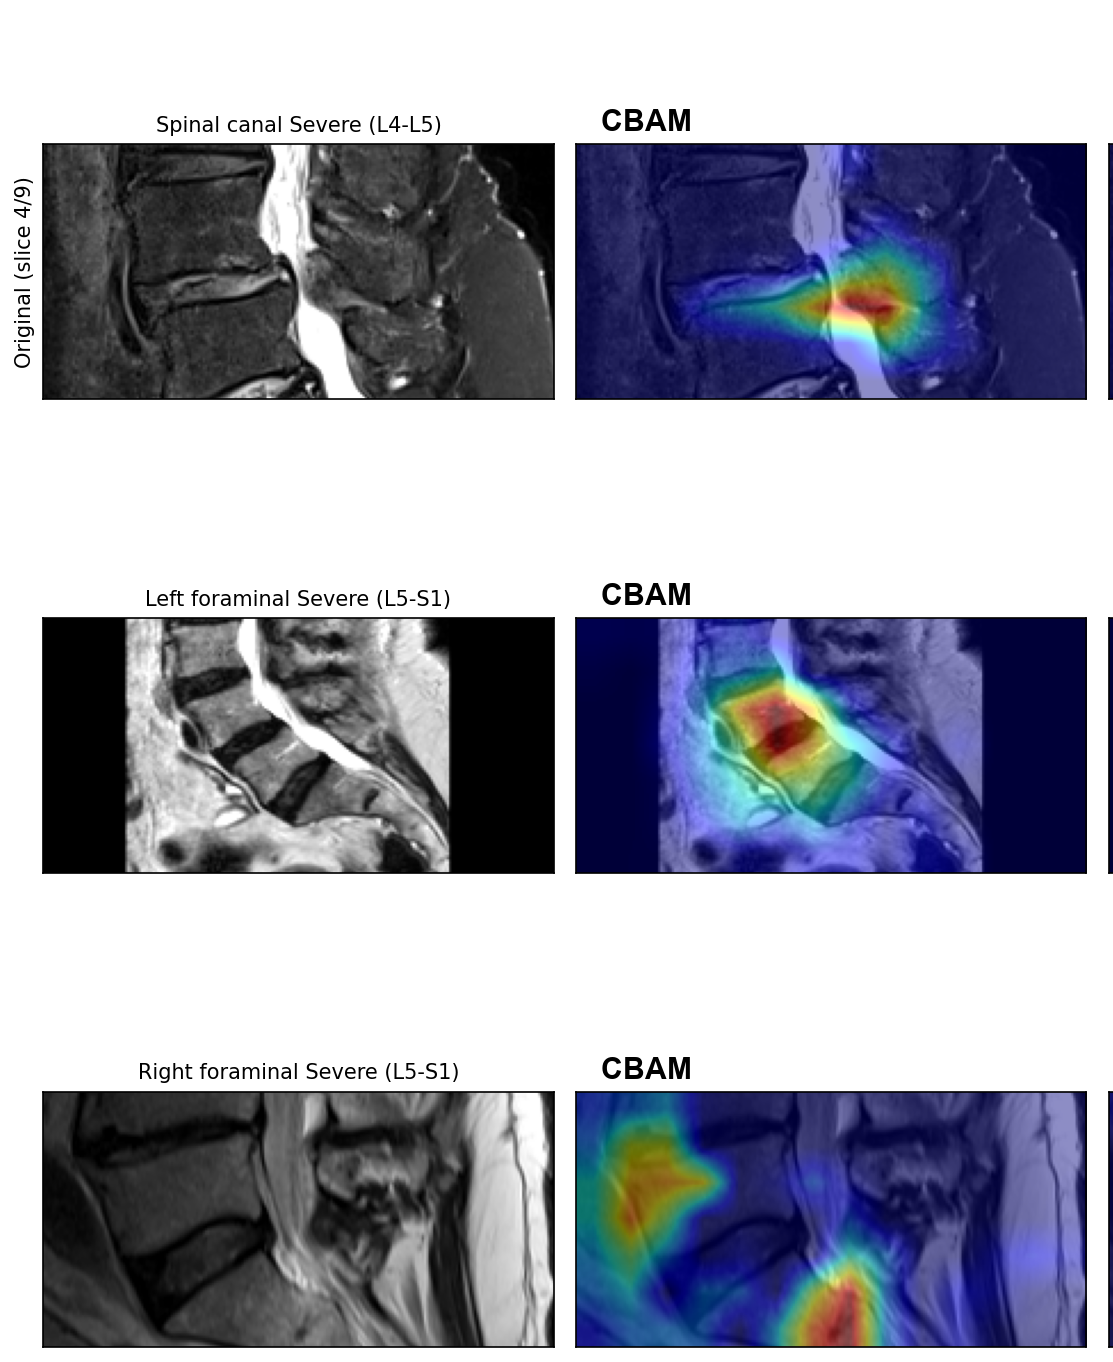
\includegraphics[height=0.72\textheight]{image/grad_cam_severe_cbam.png}
    \caption{Grad-CAM tại nhánh CBAM trên các ca Severe.}
\end{figure}
\end{frame}

\subsection{Mở rộng nhãn zero-shot}
\begin{frame}
\frametitle{Mở rộng nhãn zero-shot trên SPIDER}
\begin{columns}[t]
\column{.5\textwidth}
\small
Nhờ nhánh BiomedCLIP + text prompt, kiến trúc Hybrid dự đoán được nhãn mới chưa từng huấn luyện (zero-shot), không cần train trên SPIDER.
\begin{itemize}\small
    \item[$\rightarrow$] Baseline/CBAM không làm được vì head cố định 3 lớp.
    \item[--] Nhãn liên quan đĩa đệm chuyển giao tốt; nhãn xa ngữ nghĩa (Modic, Pfirrmann, trượt đốt sống) còn yếu.
\end{itemize}
\column{.5\textwidth}
\begin{table}
\centering
\footnotesize
\begin{tabular}{lcc}
\toprule
\textbf{Nhãn SPIDER} & \textbf{F1} & \textbf{AUC} \\
\midrule
Disc bulging        & \textbf{0.709} & 0.806 \\
Disc herniation     & 0.522 & 0.802 \\
Disc narrowing      & 0.388 & 0.836 \\
\midrule
Lower endplate      & 0.452 & 0.747 \\
Upper endplate      & 0.441 & 0.743 \\
Pfirrmann (5 lớp)   & 0.147 & 0.492 \\
Modic (4 lớp)       & 0.117 & 0.422 \\
Spondylolisthesis   & 0.030 & 0.745 \\
\midrule
\textbf{Trung bình (8)} & \textbf{0.362} & \textbf{0.699} \\
\bottomrule
\end{tabular}
\end{table}
\end{columns}
\end{frame}

\subsection{Tổng quát hóa trên SPIDER}
\begin{frame}
\frametitle{Kết quả tổng hợp trên SPIDER (có tinh chỉnh)}
\begin{table}
\centering
\small
\begin{tabular}{lcccc}
\toprule
\textbf{Chỉ số} & \textbf{SpineNetV2} & \textbf{CBAM} & \textbf{BMC-only} & \textbf{Hybrid} \\
\midrule
Mean Accuracy (\%) & \textbf{80.23} & 79.27 & 76.12 & 78.30 \\
Mean F1 (macro)    & 0.646 & 0.619 & 0.613 & \textbf{0.653} \\
Mean AUC           & 0.842 & 0.824 & 0.808 & \textbf{0.846} \\
Mean AUPRC         & \textbf{0.633} & 0.580 & 0.544 & 0.611 \\
\bottomrule
\end{tabular}
\caption{Kết quả trung bình 4 cấu hình trên SPIDER (có tinh chỉnh).}
\end{table}
\begin{itemize}
    \item[$\rightarrow$] Có tinh chỉnh, kết quả cao hơn hẳn zero-shot (Mean F1 0.653 so với 0.362).
    \item[--] SpineNetV2 và Hybrid bám sát nhau; Hybrid nhỉnh hơn về F1/AUC, SpineNetV2 nhỉnh về Accuracy/AUPRC.
\end{itemize}
\end{frame}

\begin{frame}
\frametitle{Kết quả chi tiết trên SPIDER (có tinh chỉnh)}
\begin{table}
\centering
\scriptsize
\setlength{\tabcolsep}{3.5pt}
\resizebox{\textwidth}{!}{%
\begin{tabular}{lccccccccccc}
\toprule
& \multicolumn{5}{c}{\textbf{SpineNetV2}} & & \multicolumn{5}{c}{\textbf{Hybrid}} \\
\cmidrule(lr){2-6}\cmidrule(lr){8-12}
\textbf{Nhóm bệnh} & R & P & F1 & AUC & AUPRC & & R & P & F1 & AUC & AUPRC \\
\midrule
Modic             & 0.374 & \textbf{0.383} & 0.376 & 0.731 & \textbf{0.545} & & \textbf{0.382} & 0.377 & \textbf{0.379} & \textbf{0.827} & 0.500 \\
Disc narrowing    & 0.820 & \textbf{0.828} & 0.823 & \textbf{0.927} & 0.882 & & \textbf{0.836} & 0.827 & \textbf{0.831} & 0.916 & \textbf{0.884} \\
Spondylolisthesis & 0.597 & \textbf{0.793} & \textbf{0.632} & \textbf{0.826} & \textbf{0.325} & & \textbf{0.633} & 0.607 & 0.613 & 0.815 & 0.302 \\
UP endplate       & 0.727 & 0.746 & 0.728 & 0.820 & \textbf{0.753} & & \textbf{0.753} & \textbf{0.748} & \textbf{0.749} & \textbf{0.828} & 0.751 \\
LOW endplate      & \textbf{0.754} & \textbf{0.764} & \textbf{0.757} & 0.823 & \textbf{0.775} & & 0.743 & 0.745 & 0.744 & \textbf{0.826} & 0.763 \\
Disc herniation   & 0.500 & 0.470 & 0.485 & 0.852 & \textbf{0.271} & & \textbf{0.636} & \textbf{0.592} & \textbf{0.601} & \textbf{0.860} & 0.248 \\
Disc bulging      & 0.778 & 0.779 & 0.777 & \textbf{0.874} & 0.840 & & \textbf{0.796} & \textbf{0.794} & \textbf{0.792} & 0.873 & \textbf{0.851} \\
\bottomrule
\end{tabular}}
\caption{Recall/Precision/F1/AUC/AUPRC theo từng nhóm bệnh trên SPIDER.}
\end{table}
\begin{itemize}
    \item[$\rightarrow$] Hybrid cải thiện Recall/F1/AUC ở phần lớn nhóm bệnh, rõ nhất ở Disc herniation và Disc bulging.
\end{itemize}
\end{frame}

%----------------------------------------------------------------------------------------
%	6. KẾT LUẬN
%----------------------------------------------------------------------------------------
\section{Kết luận và hướng phát triển}
{
    \begin{frame}
        \frametitle{Mục lục}
        \tableofcontents[currentsection, hideothersubsections]
    \end{frame}
}

\begin{frame}
\frametitle{Kết quả đạt được}
\begin{itemize}
    \item[--] Khảo sát và lựa chọn mô hình tham khảo cho hai giai đoạn phân vùng và đánh giá bệnh lý.
    \item[--] Đề xuất kiến trúc Hybrid CBAM + BiomedCLIP, cải thiện rõ rệt trên lớp Severe (Recall 11.5\% $\rightarrow$ 46.4\%).
    \item[--] Kiểm chứng khả năng tổng quát hóa qua transfer learning sang SPIDER.
\end{itemize}
\end{frame}

\begin{frame}
\frametitle{Hạn chế}
\begin{itemize}
    \item[--] Hai mô-đun phân vùng và đánh giá còn chạy độc lập, chưa tích hợp thành pipeline hoàn chỉnh.
    \item[--] Mô hình mới khai thác mặt cắt Sagittal, chưa dùng mặt cắt Axial.
\end{itemize}
\end{frame}

\begin{frame}
\frametitle{Kế hoạch giai đoạn Đồ án tốt nghiệp}
\begin{table}
\centering
\begin{tabular}{clc}
\toprule
\textbf{GĐ} & \textbf{Nội dung} & \textbf{Thời lượng} \\
\midrule
1 & Tích hợp pipeline end-to-end (mặt nạ định vị ROI) & 3 tuần \\
2 & Xây dựng phần mềm giao diện cho bác sĩ & 6 tuần \\
3 & Tinh chỉnh tiếp mô-đun grading & 3 tuần \\
4 & Viết Đồ án tốt nghiệp và chuẩn bị bảo vệ & 3 tuần \\
\bottomrule
\end{tabular}
\caption{Kế hoạch thực hiện trong giai đoạn Đồ án tốt nghiệp.}
\end{table}
\end{frame}

%------------------------------------------------
\begin{frame}
\huge{\centerline{Xin cảm ơn quý thầy cô đã lắng nghe!}}
\end{frame}

%----------------------------------------------------------------------------------------
\section{}
\begin{frame}[allowframebreaks]
\frametitle{Tài liệu tham khảo}
\printbibliography
\end{frame}

\appendix
\begin{frame}
\frametitle{Phụ lục: số tham số mô hình}
\begin{table}
\centering
\begin{tabular}{lcc}
\toprule
\textbf{Nhánh} & \textbf{Số tham số} & \textbf{Trạng thái} \\
\midrule
CBAM-3D ResNet-34 & 21.3M & Huấn luyện \\
BiomedCLIP ViT-B/16 & 86.2M & Đóng băng (frozen) \\
\bottomrule
\end{tabular}
\caption{Phân bổ tham số trong kiến trúc Hybrid; thời gian suy luận $\sim$66 ms/mẫu (RTX 4090).}
\end{table}
\end{frame}

\end{document}
